\documentclass[11pt]{article}



\usepackage[utf8]{inputenc} % Required for inputting international characters
\usepackage[T1]{fontenc} % Output font encoding for international characters
\usepackage{graphicx}
\usepackage{float}
\usepackage{geometry}
\usepackage{hyperref}
\usepackage{amsmath}
\usepackage{cite}
\usepackage{pdfpages}
\usepackage{caption} 
\usepackage{subcaption}
\captionsetup[table]{position=above,skip=0.7cm} 
\newcommand{\RM}[1]{\MakeUppercase{\romannumeral #1{}}}
\makeatletter
\newcommand*{\rom}[1]{\expandafter\@slowromancap\romannumeral #1@}
\makeatother

\usepackage{adjustbox}
\usepackage[german]{varioref}
\usepackage{mathpazo} % Palatino font
\usepackage[german]{babel}
\parindent0pt
\pdfinclusioncopyfonts=1

\begin{document}

\begin{titlepage} % Suppresses displaying the page number on the title page and the subsequent page counts as page 1
	\newcommand{\HRule}{\rule{\linewidth}{0.5mm}} % Defines a new command for horizontal lines, change thickness here
	
	\center % Centre everything on the page
	\vspace*{0.75cm}
%
\includegraphics[width=0.8\textwidth]{../tex/fu_logo}\\[1cm] 

%\textsc{\LARGE  Freie Universität Berlin}\\[1.5cm] % Main heading such as the name of your university/college
	
	\textsc{\Large Neurobiologie für BioinformatikerInnen: Praktikum B}\\[0.65cm] % Major heading such as course name
	
	\textsc{\large Protokoll zum 5. Praktikumstag am 04.02.2019}\\[0.65cm] % Minor heading such as course title

	\HRule\\[0.5cm]
	
	{\huge Psychophysische Experimente zum \\[0.2cm]Farbsehen}\\[0.3cm] % Title of your document
	
	\HRule\\[0.75cm]
	\textsc{\Large\bfseries Gruppe V}
	\\[0.8cm]
	
\vfill

	\begin{minipage}{0.45\textwidth}
		\begin{flushleft}
			\large
			\textit{Gruppenmitglieder}\\
			\textsc{Alia Rothkegel}\\
			\textsc{Mara Steiger}
			 % Your name
		\end{flushleft}
	\end{minipage}
	~
	\begin{minipage}{0.45\textwidth}
		\begin{flushright}
			\large \vspace{16pt}
			alia.rothkegel@fu-berlin.de\\
			mara.steiger@fu-berlin.de 
		\end{flushright}
	\end{minipage}
	
\vfill

	\begin{minipage}{0.45\textwidth}
		\begin{flushleft}
			\large
			\textit{Lehrveranstalter}\\
			Prof. Dr. P.R. \textsc{Hiesinger}\\ 
			Dr. D. \textsc{Malun}\\ 
			Prof. Dr. M. \textsc{Wernet}
		\end{flushleft}
	\end{minipage}
	~
		\begin{minipage}{0.45\textwidth}
		\begin{flushright}
			
		\end{flushright}
	\end{minipage}
\vfill
	\begin{minipage}{0.7\textwidth}
		\begin{flushleft}
			\large
			\textit{TutorInnen}\\
			\textsc{Lisa Peters}\\
			\textsc{Johannes Brüner Hammacher}\\
			\textsc{Claudia Haushalter}
		\end{flushleft}
	\end{minipage}
	~
		\begin{minipage}{0.2\textwidth}
		\begin{flushright}
			
		\end{flushright}
	\end{minipage}

	% If you don't want a supervisor, uncomment the two lines below and comment the code above
	%{\large\textit{Author}}\\
	%John \textsc{Smith} % Your name
	\vfill\vfill\vfill % Position the date 3/4 down the remaining page

	
	\vfill % Push the date up 1/4 of the remaining page
	
\end{titlepage}

%----------------------------------------------------------------------------------------
\newgeometry{top=2.5cm,bottom=2.5cm,right=4cm,left=4cm}
\section{Einleitung}


\section{Material und Methoden}
\subsection{Material}
Für diesen Versuch benötigten wir lediglich einen Computer mit den entsprechenden Programmen.
\subsection{Methoden}
\begin{enumerate}
\item \textbf{Farbenkreis} \\
Im zugehörigen Programm (\textit{farbkreis.bat}) wurden 12 Farbstimuli in verschiedenen Farben vorgegeben, die nach einem gewählten Prinzip systematisch in einem Farbkreis angeordnet werden sollten. 
\item \textbf{Farbmischung \RM{1}} \\
Unter Verwendung des Programmes \textit{rgbmon.bat} sollten die Grundfarben und zusätzlich ein mittleres Grau hergestellt werden. Die frei wählbaren Faktoren war hier die Farbmischung der Farben Rot, Grün und Blau, entsprechend den RGB-Werten ($0-100\%$). 
\item \textbf{Farbintensität} \\
In diesem Teilversuch wurde das Programm \textit{ipxl.bat} mit dem Experiment \textit{Simple colored disk} verwendet. Die Option \textit{Follow invalid colors} wurde ausgeschaltet, außerdem wurde die Anzeige von den Koordinaten für Yxy und L*a*b* ausgewählt. \\
Zunächst haben wir den Weißpunkt in beiden Farbräumen gesucht und notiert. Dann haben wir die Intensitäten so weit verringert, bis im Diagramm kein Dreieck mehr angezeigt wurde. \\
Anschließend wurden für zwei Farbtöne jeweils Farbton, Sättigung und Helligkeit variiert und die Veränderungen dokumentiert. \\
Dann wurde die Intensität des Hintergrundes variiert, dies wurde für die ursprüngliche Größe des Farbstimulus getestet und für einen verkleinerten Farbstimulus.
\item \textbf{Farbreihe} \\
In diesem Teil wurde erneut das Programm \textit{ipxl.bat} verwendet, diesmal jedoch mit dem Experiment \textit{High intensity stairs: Contrast}. \\
Die erste Farbreihe wurde mit konstanter Sättigung und Helligkeit durchgeführt, indem nur der Farbton verändert wurde. \\
Bei der zweiten Farbreihe wurde die Helligkeit verändert und entsprechend die Sättigung und der Farbton mit konstanten Werten verwendet. \\
Zuletzt wurde eine Farbreihe mit systematisch variierter Helligkeit, aber konstanter Sättigung und Farbton erstellt.

\item \textbf{Farbmischung \RM{2}} \\
In diesem Teil wurde das Programm \textit{ipxl.bat} mit dem Experiment \textit{Matching and spatial mixture} verwendet. \\
Hier wurden zwei Farbquadrate angezeigt. Die Farbe des linken Fenster konnte mit einer Farbe bestimmt werden, das rechte Fenster dagegen enthielt feine Linien aus zwei verschiedenen Farbtönen. \\
Im Versuch sollte eine Farbe links festgelegt werden, die dann auf der rechten Seite durch das Farbpaar möglichst gut nachzumischen. \\
Nachdem ein Farbpaar gefunden wurde, sollte für die gleiche Grundfarbe auf der linken Seite ein weiteres Farbpaar bestimmt werden, mit dem diese Farbe nachgemischt werden kann. 

\item \textbf{Simultaner Farbkontrast } \\
In diesem Teil wurde das Programm \textit{ipxl.bat} mit dem Experiment \textit{Simultaneos color contrast} verwendet. \\
Hier waren zwei große Farbquadrate nebeneinander, dessen Farbe unabhängig voneinander eingestellt werden konnte. In der Mitte beider Quadrate befanden sich zwei weitere, kleine Quadrate die beide die gleiche Farbe haben. \\
Es wurden für die äußeren und inneren Quadrate gesucht, sodass die Farben der inneren Flächen auf den Betrachter verschieden wirken. 

\item \textbf{Sukzessiver Farbkontrast } \\
In diesem Teil wurde das Programm \textit{ipxl.bat} mit verschiedenen Experimenten unter \textit{Adaption effects} verwendet. \\
Zunächst wurde das Modul \textit{Aftereffects and Opponent Colors}, wobei ein graues Quadrat angezeigt wurde, in dem vier weitere Quadrate angeordnet waren, jeweils eins in gelb, blau, grün und rot. \\
Die Mitte zwischen diesen Quadraten wurde vom Betrachter ca. 30 Sekunden fixiert und dann durch Klicken auf \textit{Step} die bunten Flächen entfernt. Auftretende Nachbilder wurden bei verschiedenen Entfernungen betrachtet und notiert. \\
Danach wurden doch die Module \textit{Induction}, \textit{Desaturation by Adaptation} und \textit{Hypersaturation} getestet und auftretende Nachbilder dokumentiert. 

\end{enumerate}

\section{Ergebnisse}
\subsection{Farbenkreis}
Wir haben hier die Farbstimuli nach Ähnlichkeit im Farbkreis sortiert. Ähnliche Farben sind somit nebeneinander und Komplementärfarben liegen sich gegenüber im Farbkreis. 
\begin{figure}[H]
\makebox[\textwidth][c]{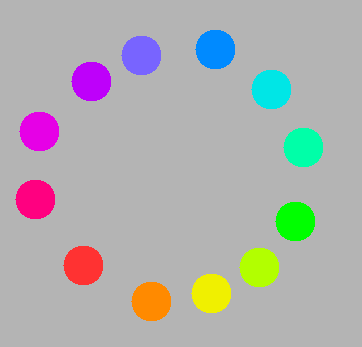
\includegraphics[width=0.7\textwidth]{a2/kreis}}
\caption{Die Abbildung zeigt den von uns erstellten Farbkreis durch die Anordnung der Farbstimuli nach dem oben beschriebenen Prinzip.}
\label{farbkreis}
\end{figure}


\subsection{Farbmischung \rom{1}}
Die erste drei Farben (Rot, Grün, Blau) sind Grundfarben und konnten einfach durch die Einstellung des entsprechenden Reglers auf $100\%$ hergestellt werden (siehe Abbildungen \ref{rotmix}-\ref{blaumix}).  \\
Gelb wurde durch die Kombination von Rot ($100\%$) und Grün ($100\%$) hergestellt. 
Magenta wurde durch die Kombination von Rot ($100\%$) und Blau ($100\%$) hergestellt. 
Cyan wurde durch die Kombination von Blau ($100\%$) und Grün ($100\%$) hergestellt.  \\
Die Mischung von mittlerem Grau wurde durch die Einstellung der RGB-Werte drei Farben auf $50\%$ erreicht. \\
Schwarz wurde durch die Einstellung auf $0\%$ aller RGB-Werte beobachtet. \\

\makebox[\textwidth][c]{
\begin{minipage}[t]{0.6\textwidth} 
\begin{figure}[H]
\makebox[\textwidth][c]{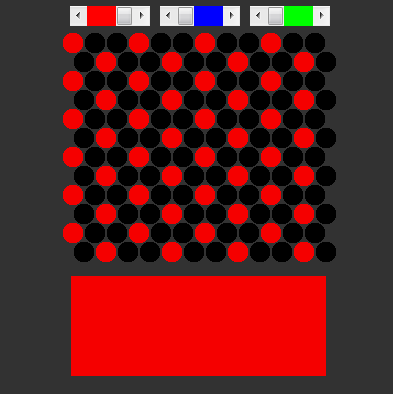
\includegraphics[width=\textwidth]{a3/rot}}
\caption{Hier ist die Herstellung der Farbe \textit{Rot} mittels Farmischung der RGB-Farben zu sehen.}
\label{rotmix}
\end{figure}
\end{minipage} 
\hfill \hspace{1.5cm}
\begin{minipage}[t]{0.6\textwidth} 
\vspace{0pt}
\begin{figure}[H]
\makebox[\textwidth][c]{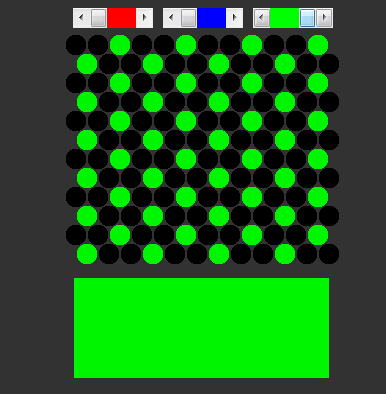
\includegraphics[width=\textwidth]{a3/gruen}}
\caption{Hier ist die Herstellung der Farbe \textit{Grün} mittels Farmischung der RGB-Farben zu sehen.}
\label{gruenmix}
\end{figure}
\end{minipage} }

\makebox[\textwidth][c]{
\begin{minipage}[t]{0.6\textwidth} 
\begin{figure}[H]
\makebox[\textwidth][c]{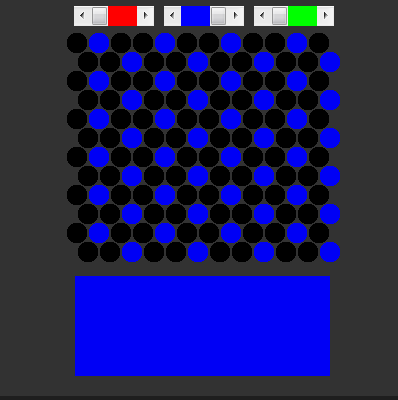
\includegraphics[width=\textwidth]{a3/blau}}
\caption{Hier ist die Herstellung der Farbe \textit{Blau} mittels Farmischung der RGB-Farben zu sehen.}
\label{blaumix}
\end{figure}
\end{minipage} 
\hfill \hspace{1.5cm}
\begin{minipage}[t]{0.6\textwidth} 
\vspace{0pt}
\begin{figure}[H]
\makebox[\textwidth][c]{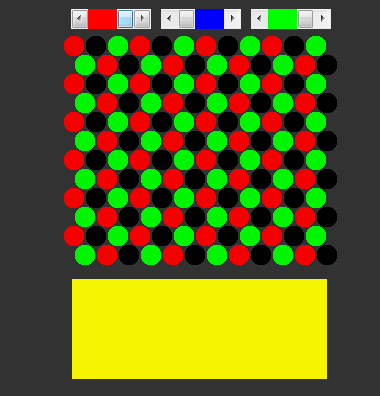
\includegraphics[width=\textwidth]{a3/gelb}}
\caption{Hier ist die Herstellung der Farbe \textit{Gelb} mittels Farmischung der RGB-Farben zu sehen.}
\label{gelbmix}
\end{figure}
\end{minipage} }

\makebox[\textwidth][c]{
\begin{minipage}[t]{0.6\textwidth} 
\begin{figure}[H]
\makebox[\textwidth][c]{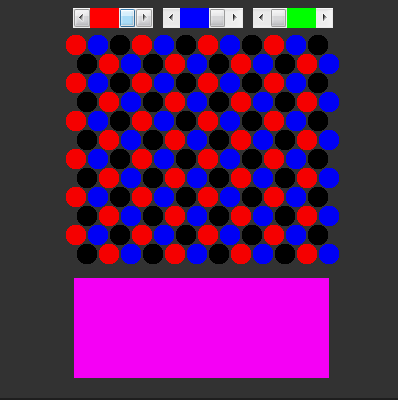
\includegraphics[width=\textwidth]{a3/magenta}}
\caption{Hier ist die Herstellung der Farbe \textit{Rot} mittels Farmischung der RGB-Farben zu sehen.}
\label{magentamax}
\end{figure}
\end{minipage} 
\hfill \hspace{1.5cm}
\begin{minipage}[t]{0.6\textwidth} 
\vspace{0pt}
\begin{figure}[H]
\makebox[\textwidth][c]{\includegraphics[width=\textwidth]{a3/Cyan}}
\caption{Hier ist die Herstellung der Farbe \textit{Grün} mittels Farmischung der RGB-Farben zu sehen.}
\label{cyanmix}
\end{figure}
\end{minipage} }

\makebox[\textwidth][c]{
\begin{minipage}[t]{0.6\textwidth} 
\vspace{0pt}
\begin{figure}[H]
\makebox[\textwidth][c]{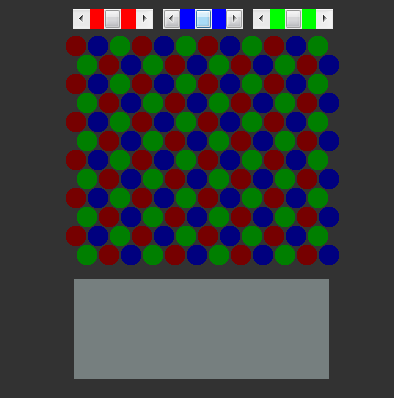
\includegraphics[width=\textwidth]{a3/grau}}
\caption{Hier ist die Herstellung der Farbe \textit{Grau} mittels Farmischung der RGB-Farben zu sehen.}
\label{graumix}
\end{figure}
\end{minipage}
\hfill \hspace{1.5cm}
\begin{minipage}[t]{0.6\textwidth} 
\begin{figure}[H]
\makebox[\textwidth][c]{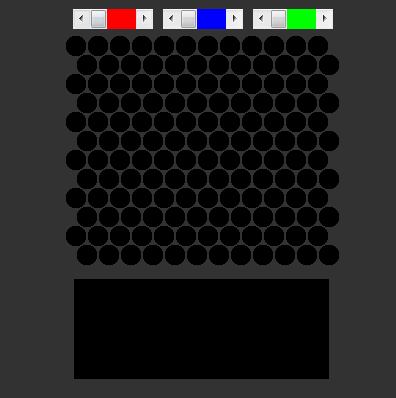
\includegraphics[width=\textwidth]{a3/schwarz}}
\caption{Hier ist die Herstellung der Farbe \textit{Schwarz} mittels Farmischung der RGB-Farben zu sehen.}
\label{schwarzmix}
\end{figure}
\end{minipage}  }



\subsection{Farbintentität}
Der Weißpunkt hat im Yxy-Raum die Koordinaten $(100,0.307,0.347)$ und im L*a*b*-Farbraum die Koordinaten (100,0,0) (siehe Abbildung \ref{weisspunkt}). 

\begin{figure}[H]
\makebox[1\textwidth][c]{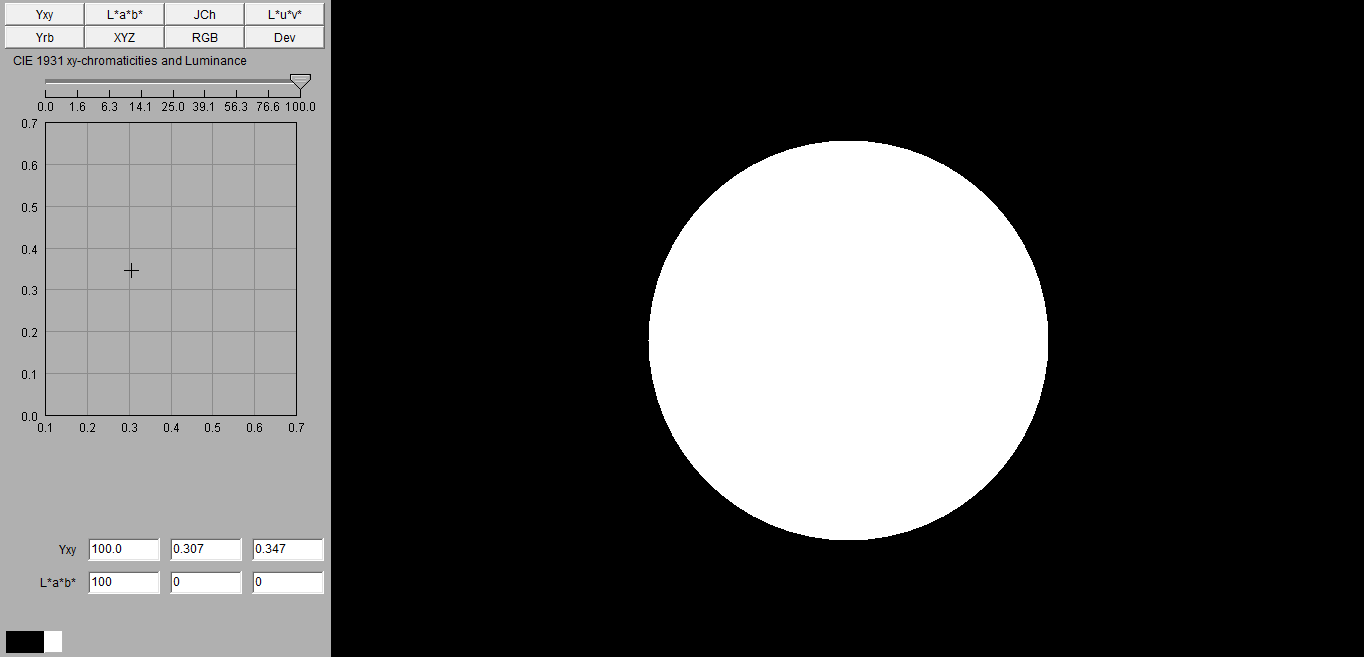
\includegraphics[width=1.3\textwidth]{a4/xyx2}}
\caption{In dem Screenshot ist zu sehen, wo der Weißpunkt im Yxy- und im Farbraum liegt.}
\label{weisspunkt}
\end{figure}



\makebox[\textwidth][c]{
\begin{minipage}[t]{0.6\textwidth} 
\vspace{0pt}
\begin{figure}[H]
\makebox[\textwidth][c]{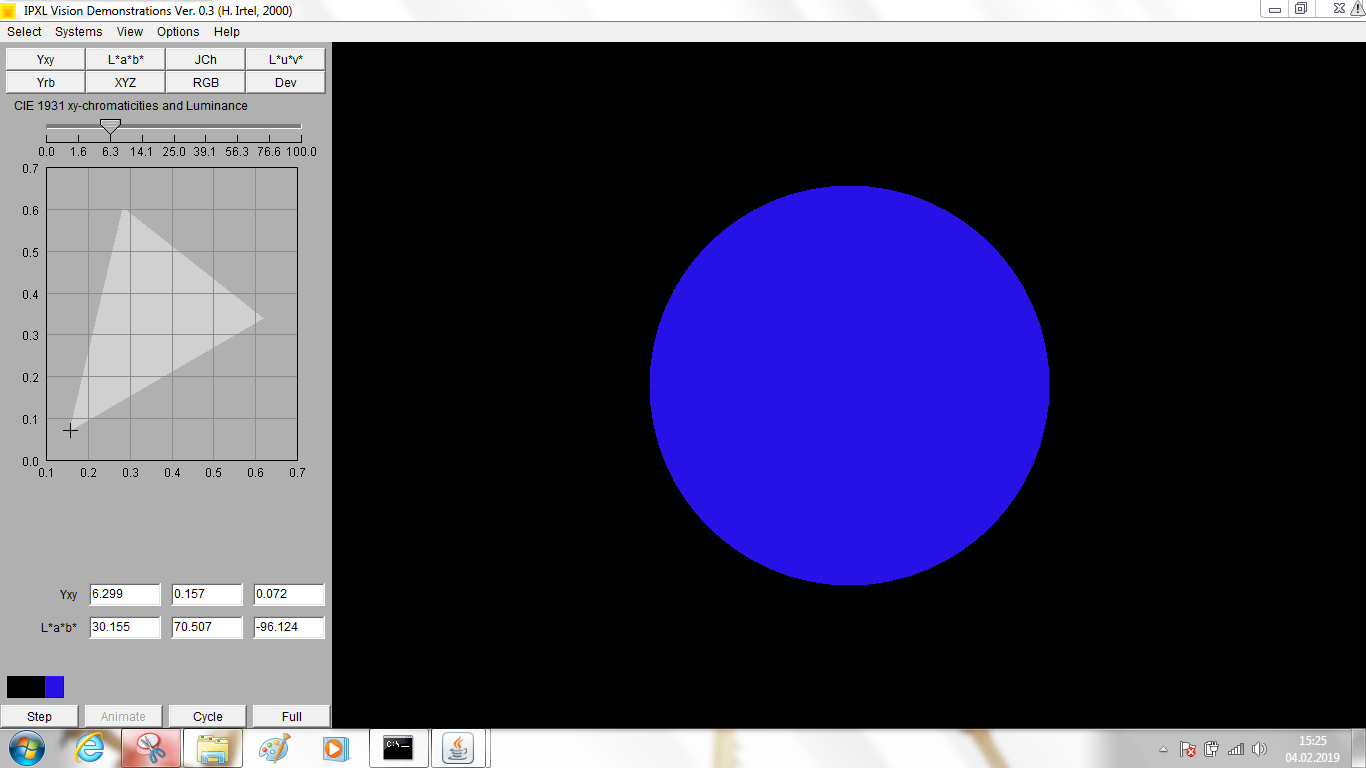
\includegraphics[width=\textwidth]{a4/blau1}}
\caption{Hier ist die Herstellung der Farbe \textit{Grau} mittels Farmischung der RGB-Farben zu sehen.}
\label{graumix}
\end{figure}
\end{minipage}
\hfill \hspace{1.5cm}
\begin{minipage}[t]{0.6\textwidth} 
\begin{figure}[H]
\makebox[\textwidth][c]{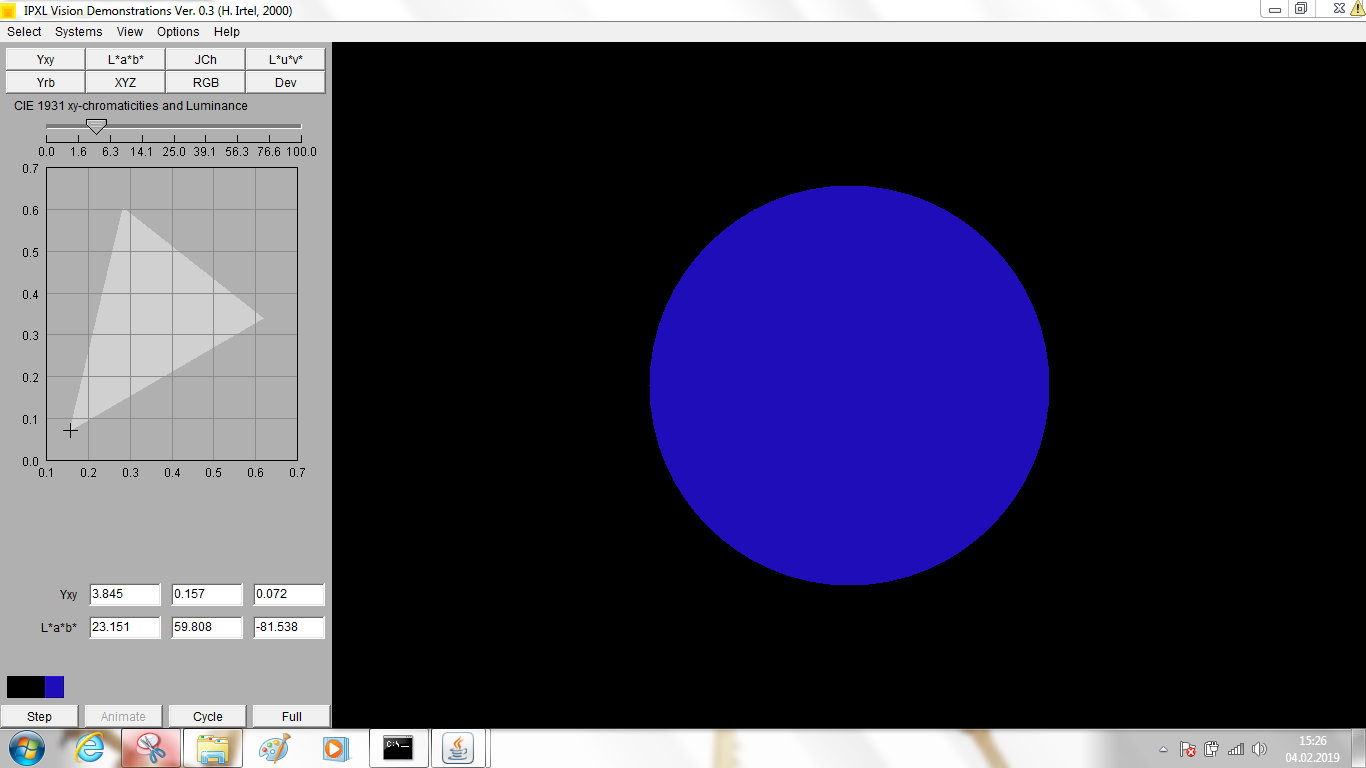
\includegraphics[width=\textwidth]{a4/blau2}}
\caption{Hier ist die Herstellung der Farbe \textit{Schwarz} mittels Farmischung der RGB-Farben zu sehen.}
\label{schwarzmix}
\end{figure}
\end{minipage}}






\subsection{Farbenreihe}
Um die Farbreihe zu erhalten, in der nur der Farbton geändert werden soll, aber die Sättigung und Helligkeit gleich bleiben sollen, haben wir Punkte auf einem imaginären Kreis um den Weißpunkt gewählt. Denn die Sättigung wird über die Entfernung zum Weißpunkt definiert, sodass alle Punkte den gleichen Abstand zu ihm haben müssen, folglich liegen sie auf einem Kreis. (siehe Abbildung \ref{farbton_reihe})
\begin{figure}[H]
\makebox[1\textwidth][c]{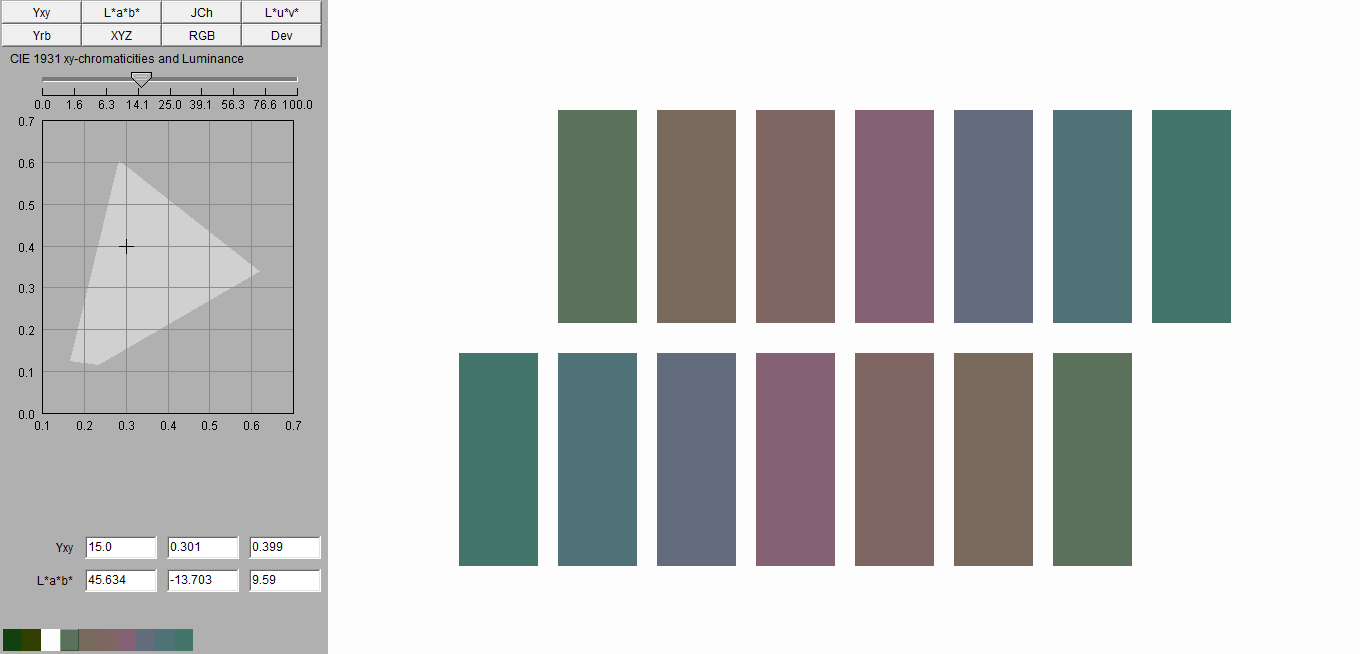
\includegraphics[width=1.3\textwidth]{a5/farbton}}
\caption{Hier ist die Farbreihe mit Änderung des Farbtons zu sehen (Sättigung und Helligkeit konstant).}
\label{farbton_reihe}
\end{figure}


Die Farbreihe mit Variabilität der Helligkeit bei Konstanz der anderen Werte wurden einfach durch die Änderung der Y Koordinate (Intensität) erzeugt. Angefangen bei einem Wert von $80$ links haben wir die Helligkeit sukzessive um $10$ verringert nach rechts (bezogen auf die obere Reihe).  (siehe Abbildung \ref{helligkeit_reihe})
\begin{figure}[H]
\makebox[1\textwidth][c]{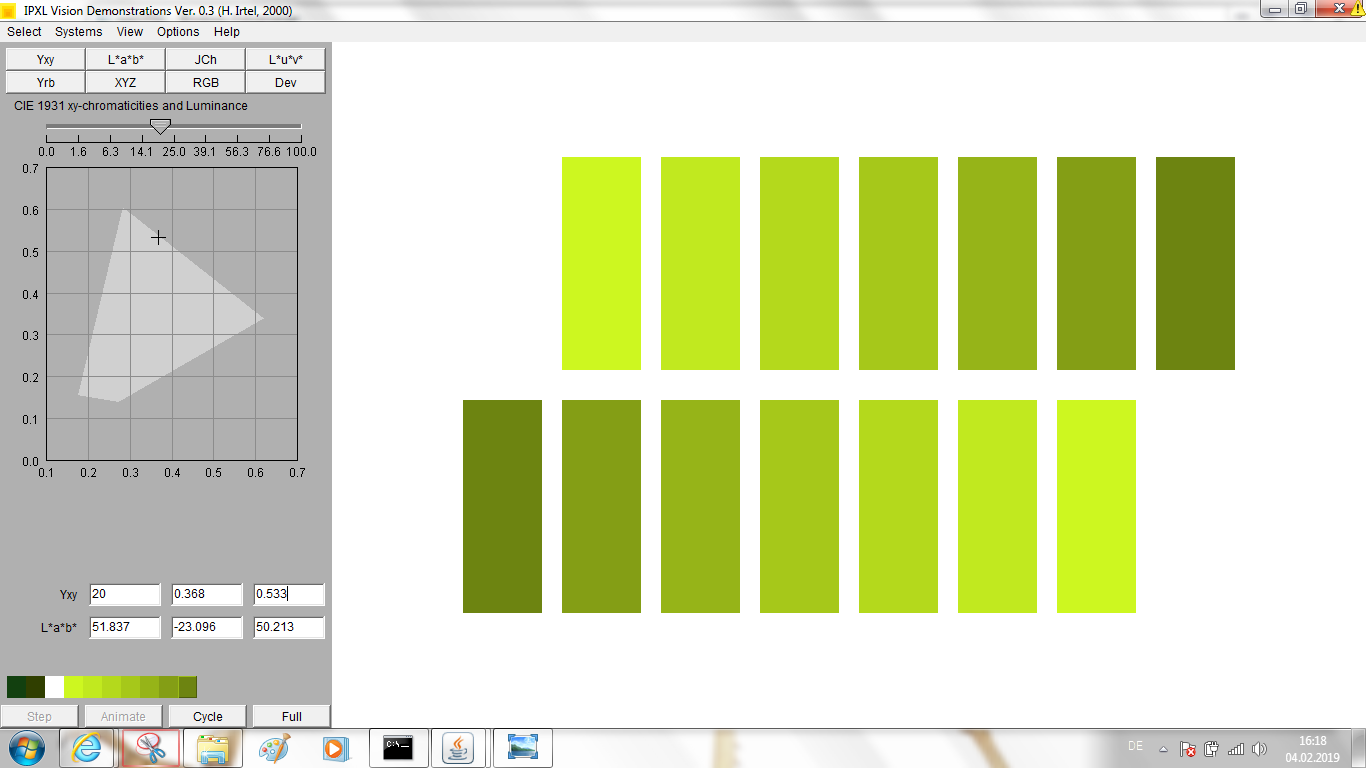
\includegraphics[width=1.3\textwidth]{a5/helligkeit2}}
\caption{Hier ist die Farbreihe mit Änderung der Helligkeit zu sehen (Sättigung und Farbton konstant).}
\label{helligkeit_reihe}
\end{figure}

Die letzte Farbreihe mit Änderungen der Sättigung bei gleichbleibendem Farbton und gleicher Helligkeit haben wir erzeugt, indem wir ausgehend von dem Farbpunkt für Grün in der Ecke des Farbdreiecks (bei Helligkeit $7$) Punkte auf der Geraden zum Weißpunkt gewählt haben. (siehe Abbildung \ref{saettigung_reihe})
\begin{figure}[H]
\makebox[1\textwidth][c]{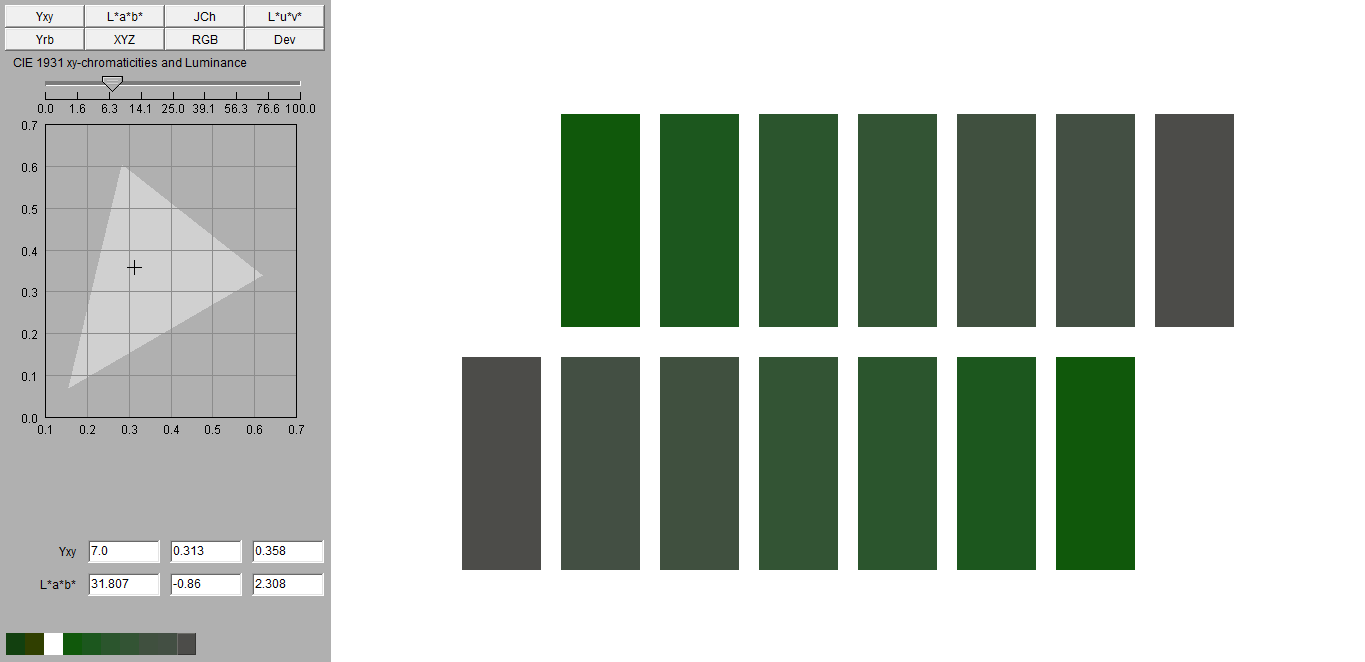
\includegraphics[width=1.3\textwidth]{a5/saettigung}}
\caption{Hier ist die Farbreihe mit Änderung des Sättigung zu sehen (Farbton und Helligkeit konstant).}
\label{saettigung_reihe}
\end{figure}

\subsection{Farbmischung \rom{2}}
Für die linke Fläche haben die Farbe mit dem Yxy-Koordinaten $(20,0.3,0.3)$ gewählt. \\
Um im rechten Fenster einen möglichst ähnlichen Farbton nachzumischen haben wir die Farben mit den Koordinaten $(20,0.258, 0.511)$ (grünlich) und $(20,0.325, 0.191)$ (pink) gewählt. 


\begin{figure}[H]
\makebox[1\textwidth][c]{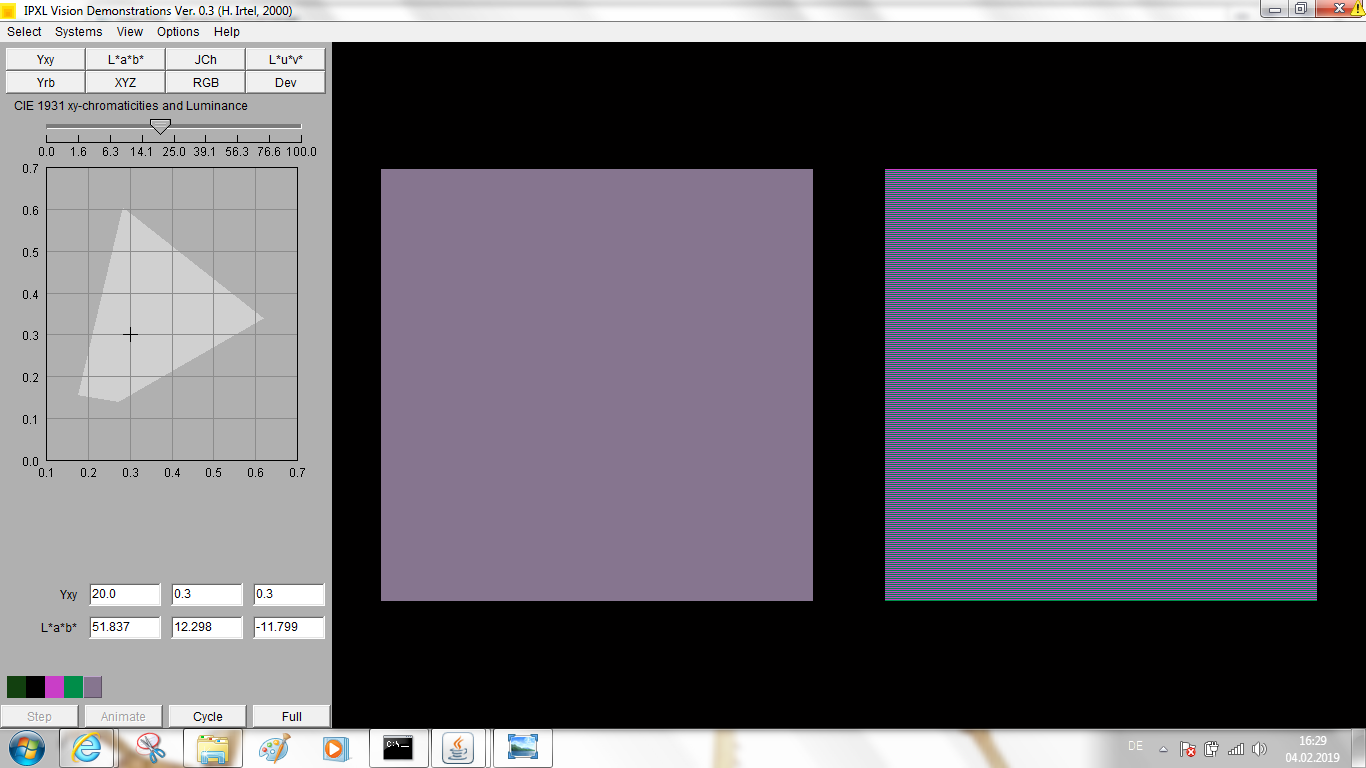
\includegraphics[width=1.3\textwidth]{a6/meta1}}
\caption{Zu sehen ist die Nachmischung der Musterfarbe (links) mit dem ersten Farbpaar (rechts) aus grün und pink.}
\label{meta1}
\end{figure}


Das zweite Farbpaar, mit dem wir die Farbe im linken Fenster nachgemischt haben, hatte die Koordinaten $(20,0.523, 0.392)$ (beige) und $(20,0.184, 0.196)$ (blau). 

\begin{figure}[H]
\makebox[1\textwidth][c]{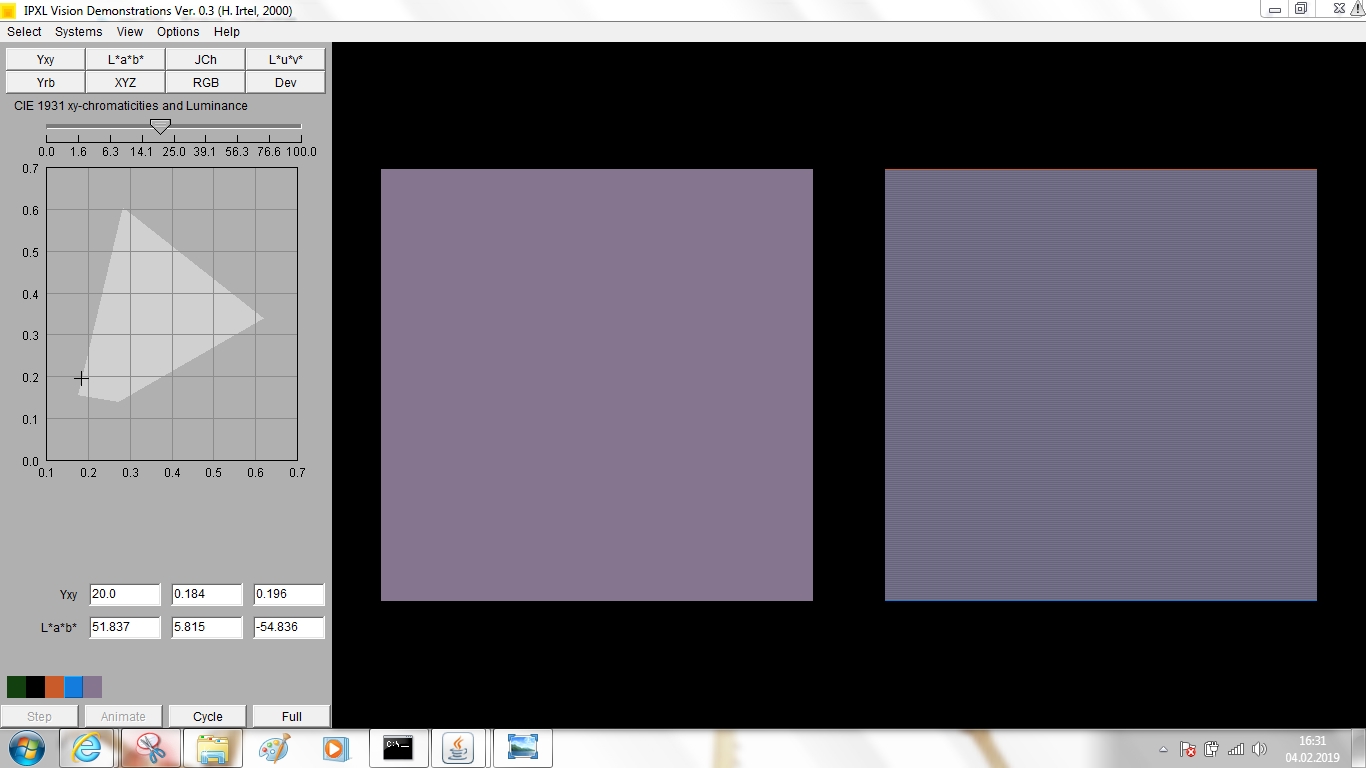
\includegraphics[width=1.3\textwidth]{a6/meta2}}
\caption{Zu sehen ist die Nachmischung der Musterfarbe (links) mit dem zweiten Farbpaar (rechts) aus beige und blau.}
\label{meta2}
\end{figure}

\subsection{Simultaner Farbkontrast}
Der simultane Farbkontrast wird besonders deutlich, wenn man für die äußere, große Fläche einmal eine sehr helle und bei der anderen Fläche eine sehr dunkle Farbe wählt. Außerdem sollten die inneren Flächen auch eher einen hellen Farbton haben. 

\begin{figure}[H]
\makebox[1\textwidth][c]{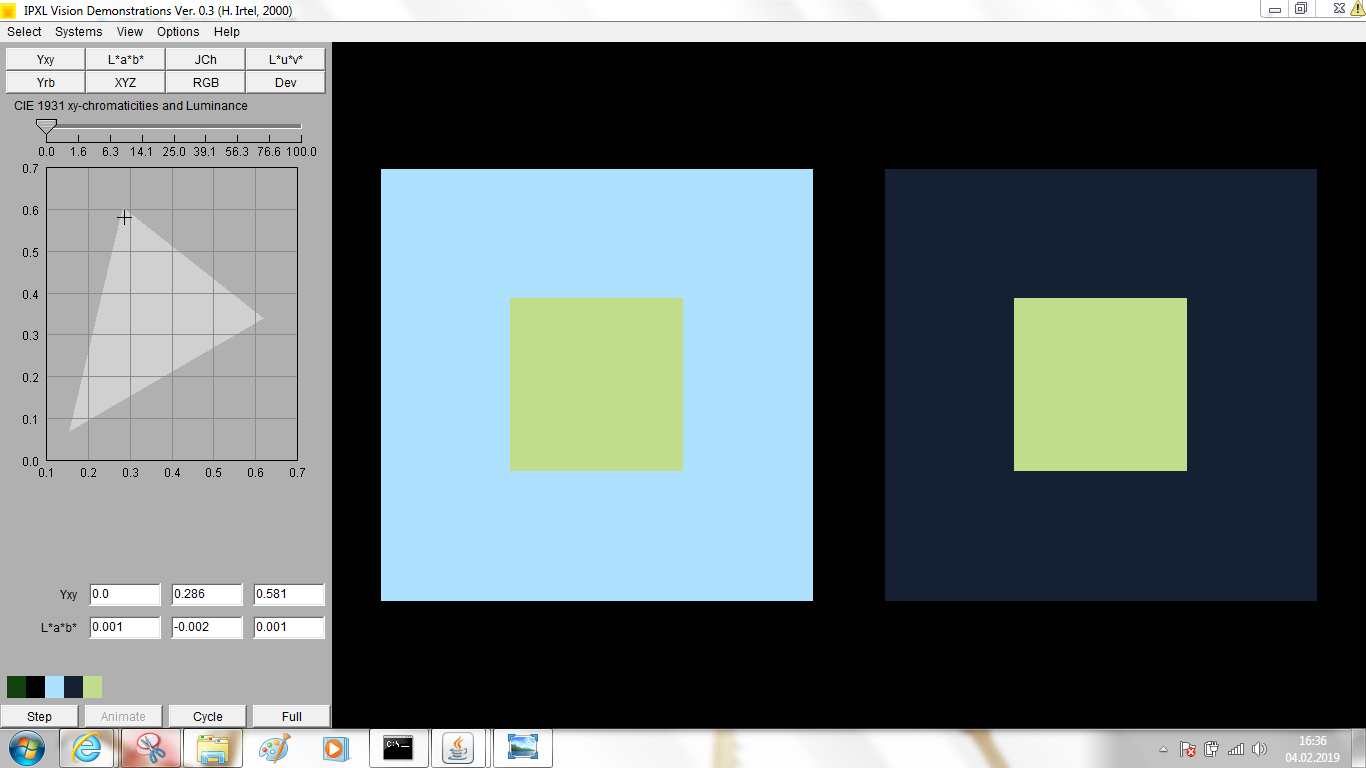
\includegraphics[width=1.3\textwidth]{a7/kontrast}}
\caption{Hier ist die Kombination von unseren ausgewählten Farben für die Simulation des simultanen Farbkonstrastes zu sehen. Links erscheint das innere Quadrat durch die hellere Umgebung dunkler als in der rechten, dunklen Fläche. Außerdem wirken die Übergänge links verschwommener, als beim starken Kontrast auf der rechten Seite.}
\label{meta2}
\end{figure}

\subsection{Sukzessiver Farbkontrast}

\section{Diskussion}


\end{document}